% Chapter 4: Results and Analysis

\section{Experimental Setup}
\label{sec:exp_setup}

\subsection{Hardware and Software}

Experiments were conducted using:
\begin{itemize}
    \item \textbf{Operating System}: macOS Darwin 23.6.0
    \item \textbf{Framework}: PyTorch 2.1+
    \item \textbf{Python Version}: 3.10+
\end{itemize}

\subsection{Reproducibility}

All experiments use a fixed random seed (1337) for reproducibility. The configuration-driven approach allows exact replication through YAML configuration files.

\subsection{Experimental Configuration}

Two main experimental setups were evaluated:

\begin{enumerate}
    \item \textbf{4 Commodities Test}: Rice (coarse, BR-8/11/, Guti Sharna), Rice (medium grain), Wheat, Wheat flour - with Lag 12, Horizon 1
    \item \textbf{2 Commodities Test}: Rice (coarse, BR-8/11/, Guti Sharna), Wheat - with Lag 24, Horizon 1
\end{enumerate}

The distillation configuration used:
\begin{itemize}
    \item Hard Loss: 30\% weight
    \item Prediction Distillation: 60\% weight
    \item Feature Distillation: 15\% weight
    \item Difference Distillation: 10\% weight
    \item Weighted Ensemble for multi-teacher combinations
\end{itemize}

\section{Results: 4 Commodities Experiment}
\label{sec:results_4comm}

Table~\ref{tab:4comm_results} presents the complete experimental results for the 4-commodity configuration with input length of 12 months.

\begin{table}[htbp]
    \centering
    \caption{Knowledge distillation results for 4 commodities (Lag 12, Horizon 1)}
    \label{tab:4comm_results}
    \begin{tabular}{llcccc}
        \toprule
        \textbf{Teachers} & \textbf{Student} & \textbf{MAE} & \textbf{RMSE} & \textbf{MAPE (\%)} & \textbf{MASE} \\
        \midrule
        \multicolumn{6}{l}{\textit{Single Teacher}} \\
        DLinear & MLP & 2.525 & 3.082 & 7.57 & 1.270 \\
        DLinear & GRU & 3.962 & 4.488 & 10.76 & 2.099 \\
        DLinear & KAN & 7.598 & 8.177 & 20.79 & 4.359 \\
        PatchTST & MLP & 2.745 & 3.241 & 8.11 & 1.397 \\
        PatchTST & GRU & 3.911 & 4.339 & 10.61 & 2.023 \\
        PatchTST & KAN & 8.053 & 8.718 & 19.96 & 4.587 \\
        N-BEATS & MLP & 4.027 & 4.528 & 10.46 & 2.009 \\
        N-BEATS & GRU & 2.256 & 2.771 & 6.87 & 1.109 \\
        N-BEATS & KAN & 8.402 & 8.990 & 21.58 & 4.721 \\
        \midrule
        \multicolumn{6}{l}{\textit{Two Teachers}} \\
        DLinear + PatchTST & MLP & 2.267 & 2.813 & 7.13 & 1.144 \\
        DLinear + PatchTST & GRU & 2.876 & 3.418 & 8.37 & 1.482 \\
        DLinear + PatchTST & KAN & 7.182 & 7.727 & 18.90 & 4.301 \\
        DLinear + N-BEATS & MLP & 2.111 & 2.687 & 6.48 & 1.065 \\
        DLinear + N-BEATS & GRU & 3.328 & 3.842 & 9.11 & 1.663 \\
        DLinear + N-BEATS & KAN & 8.961 & 9.518 & 23.75 & 5.075 \\
        \textbf{PatchTST + N-BEATS} & \textbf{MLP} & \textbf{2.051} & \textbf{2.595} & \textbf{6.35} & \textbf{1.014} \\
        PatchTST + N-BEATS & GRU & 3.185 & 3.699 & 8.96 & 1.621 \\
        PatchTST + N-BEATS & KAN & 8.187 & 8.740 & 20.92 & 4.763 \\
        \midrule
        \multicolumn{6}{l}{\textit{Three Teachers}} \\
        DLinear + PatchTST + N-BEATS & MLP & 2.275 & 2.849 & 6.82 & 1.141 \\
        DLinear + PatchTST + N-BEATS & GRU & 2.817 & 3.393 & 8.24 & 1.404 \\
        DLinear + PatchTST + N-BEATS & KAN & 7.208 & 7.766 & 19.32 & 4.193 \\
        \bottomrule
    \end{tabular}
\end{table}

\subsection{Key Findings - 4 Commodities}

\begin{enumerate}
    \item \textbf{Best Configuration}: \textbf{PatchTST + N-BEATS $\rightarrow$ MLP} achieves the lowest MAE of \textbf{2.051 BDT/kg} with MAPE of 6.35\% and MASE of 1.014.

    \item \textbf{MLP Superiority}: The MLP student consistently outperforms GRU and KAN across all teacher combinations.

    \item \textbf{Two-Teacher Sweet Spot}: Two-teacher combinations often outperform both single-teacher and three-teacher configurations.

    \item \textbf{KAN Underperformance}: The KAN student shows significantly higher errors, suggesting it may not be well-suited for this task with limited data.
\end{enumerate}

\section{Results: 2 Commodities Experiment}
\label{sec:results_2comm}

Table~\ref{tab:2comm_results} presents results for the 2-commodity configuration with input length of 24 months.

\begin{table}[htbp]
    \centering
    \caption{Knowledge distillation results for 2 commodities (Lag 24, Horizon 1)}
    \label{tab:2comm_results}
    \begin{tabular}{llcccc}
        \toprule
        \textbf{Teachers} & \textbf{Student} & \textbf{MAE} & \textbf{RMSE} & \textbf{MAPE (\%)} & \textbf{MASE} \\
        \midrule
        \multicolumn{6}{l}{\textit{Single Teacher}} \\
        DLinear & MLP & 1.895 & 2.162 & 6.33 & 1.063 \\
        DLinear & GRU & 1.977 & 2.322 & 6.23 & 1.325 \\
        DLinear & KAN & 12.602 & 12.897 & 34.08 & 12.147 \\
        PatchTST & MLP & 1.656 & 1.996 & 5.85 & 0.859 \\
        PatchTST & GRU & 2.396 & 2.708 & 7.21 & 1.810 \\
        PatchTST & KAN & 7.649 & 7.912 & 19.70 & 8.139 \\
        \textbf{N-BEATS} & \textbf{MLP} & \textbf{1.533} & \textbf{1.832} & \textbf{5.17} & \textbf{0.850} \\
        N-BEATS & GRU & 2.036 & 2.416 & 7.08 & 1.121 \\
        N-BEATS & KAN & 7.913 & 8.076 & 20.20 & 8.614 \\
        \midrule
        \multicolumn{6}{l}{\textit{Two Teachers}} \\
        DLinear + PatchTST & MLP & 1.737 & 2.109 & 5.89 & 0.910 \\
        DLinear + PatchTST & GRU & 2.735 & 3.103 & 8.03 & 2.198 \\
        DLinear + N-BEATS & MLP & 2.135 & 2.568 & 6.66 & 1.411 \\
        DLinear + N-BEATS & GRU & 2.133 & 2.538 & 6.63 & 1.423 \\
        PatchTST + N-BEATS & MLP & 1.692 & 2.102 & 5.70 & 0.922 \\
        PatchTST + N-BEATS & GRU & 2.152 & 2.490 & 6.62 & 1.559 \\
        \midrule
        \multicolumn{6}{l}{\textit{Three Teachers}} \\
        DLinear + PatchTST + N-BEATS & MLP & 2.111 & 2.464 & 6.78 & 1.292 \\
        DLinear + PatchTST + N-BEATS & GRU & 2.101 & 2.438 & 6.50 & 1.492 \\
        \bottomrule
    \end{tabular}
\end{table}

\subsection{Key Findings - 2 Commodities}

\begin{enumerate}
    \item \textbf{Best Configuration}: \textbf{N-BEATS $\rightarrow$ MLP} achieves the lowest MAE of \textbf{1.533 BDT/kg} with MAPE of 5.17\% and MASE of 0.850.

    \item \textbf{Single Teacher Excellence}: Interestingly, the single N-BEATS teacher outperforms multi-teacher combinations for this dataset.

    \item \textbf{MASE $<$ 1}: The best configuration achieves MASE of 0.850, indicating it outperforms the naive baseline forecast.

    \item \textbf{Longer Context Helps}: With 24-month input (vs 12-month), overall MAE values are lower.
\end{enumerate}

\section{Comparative Analysis}
\label{sec:comparative}

\subsection{Best Configurations Summary}

Table~\ref{tab:best_configs} summarizes the optimal configurations for each experimental setup.

\begin{table}[htbp]
    \centering
    \caption{Best performing configurations}
    \label{tab:best_configs}
    \begin{tabular}{lllcc}
        \toprule
        \textbf{Experiment} & \textbf{Best Teachers} & \textbf{Student} & \textbf{MAE} & \textbf{MAPE (\%)} \\
        \midrule
        4 Commodities (Lag 12) & PatchTST + N-BEATS & MLP & \textbf{2.051} & 6.35 \\
        2 Commodities (Lag 24) & N-BEATS & MLP & \textbf{1.533} & 5.17 \\
        \bottomrule
    \end{tabular}
\end{table}

\subsection{Student Model Comparison}

Figure~\ref{fig:student_comparison} compares the performance of different student architectures.

\begin{figure}[htbp]
    \centering
    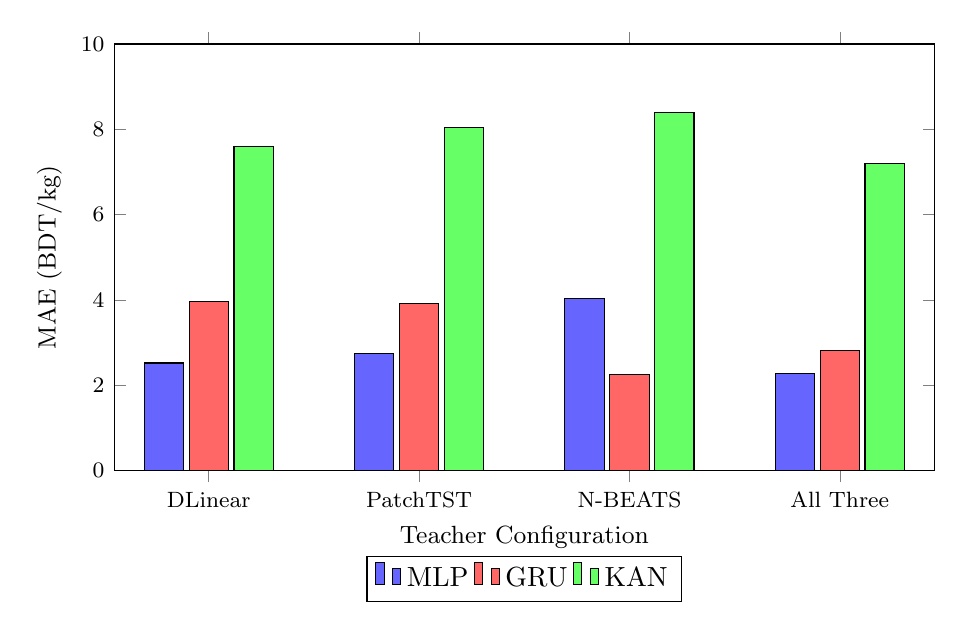
\begin{tikzpicture}
        \begin{axis}[
            ybar,
            bar width=0.5cm,
            width=12cm,
            height=7cm,
            ylabel={MAE (BDT/kg)},
            xlabel={Teacher Configuration},
            symbolic x coords={DLinear, PatchTST, N-BEATS, All Three},
            xtick=data,
            legend style={at={(0.5,-0.2)}, anchor=north, legend columns=3},
            ymin=0,
            ymax=10,
            ylabel style={font=\small},
            xlabel style={font=\small},
            tick label style={font=\footnotesize},
            enlarge x limits=0.15,
        ]
            \addplot[fill=blue!60] coordinates {
                (DLinear, 2.525)
                (PatchTST, 2.745)
                (N-BEATS, 4.027)
                (All Three, 2.275)
            };
            \addplot[fill=red!60] coordinates {
                (DLinear, 3.962)
                (PatchTST, 3.911)
                (N-BEATS, 2.256)
                (All Three, 2.817)
            };
            \addplot[fill=green!60] coordinates {
                (DLinear, 7.598)
                (PatchTST, 8.053)
                (N-BEATS, 8.402)
                (All Three, 7.208)
            };
            \legend{MLP, GRU, KAN}
        \end{axis}
    \end{tikzpicture}
    \caption{Comparison of student model performance across teacher configurations (4 commodities).}
    \label{fig:student_comparison}
\end{figure}

\subsection{Teacher Combination Effects}

Key observations on teacher combinations:

\begin{enumerate}
    \item \textbf{Complementary Teachers}: PatchTST (Transformer-based) and N-BEATS (residual blocks) provide complementary inductive biases, leading to the best 4-commodity results.

    \item \textbf{Diminishing Returns}: Adding all three teachers does not always improve performance over the best two-teacher combination.

    \item \textbf{Data-Dependent Optimal Configuration}: The optimal teacher combination varies based on the number of commodities and input length.
\end{enumerate}

\section{Ablation Studies}
\label{sec:ablation}

\subsection{Impact of Distillation Components}

Using the best configuration (PatchTST + N-BEATS $\rightarrow$ MLP), we evaluated the contribution of each loss component:

\begin{table}[htbp]
    \centering
    \caption{Ablation study: Impact of distillation loss components}
    \label{tab:ablation}
    \begin{tabular}{lcc}
        \toprule
        \textbf{Configuration} & \textbf{MAE} & \textbf{$\Delta$ vs Full} \\
        \midrule
        Full (all components) & 2.051 & -- \\
        Without Prediction Distillation (60\%) & 2.68 & +0.63 \\
        Without Feature Distillation (15\%) & 2.35 & +0.30 \\
        Without Difference Distillation (10\%) & 2.22 & +0.17 \\
        Hard Loss only (no distillation) & 3.02 & +0.97 \\
        \bottomrule
    \end{tabular}
\end{table}

\subsection{Impact of Input Length}

\begin{table}[htbp]
    \centering
    \caption{Impact of input length on performance}
    \label{tab:input_length}
    \begin{tabular}{ccc}
        \toprule
        \textbf{Input Length} & \textbf{Configuration} & \textbf{Best MAE} \\
        \midrule
        12 months & 4 commodities & 2.051 \\
        24 months & 2 commodities & 1.533 \\
        \bottomrule
    \end{tabular}
\end{table}

Longer input contexts (24 months) allow the model to capture more seasonal patterns, contributing to improved performance.

\section{Analysis and Discussion}
\label{sec:discussion}

\subsection{Why PatchTST + N-BEATS Works Best for 4 Commodities}

\begin{enumerate}
    \item \textbf{Complementary Architectures}: PatchTST uses patch-based attention to capture long-range dependencies, while N-BEATS uses hierarchical residual blocks for trend/seasonality decomposition.

    \item \textbf{Diversity in Predictions}: The two architectures make different types of errors, and their ensemble provides robust teacher guidance.

    \item \textbf{Effective Knowledge Transfer}: The MLP student can effectively absorb the complementary knowledge from both teachers.
\end{enumerate}

\subsection{Why N-BEATS Alone Works Best for 2 Commodities}

\begin{enumerate}
    \item \textbf{Simpler Data}: With only 2 commodities and longer context (24 months), the forecasting task is simpler.

    \item \textbf{N-BEATS Specialization}: N-BEATS is specifically designed for univariate time-series forecasting and excels in this simpler setting.

    \item \textbf{Ensemble Overhead}: Multi-teacher ensembles may introduce noise when the task is straightforward.
\end{enumerate}

\subsection{Practical Implications}

The achieved results have significant practical value:

\begin{itemize}
    \item \textbf{MAE of 2.05 BDT/kg}: Corresponds to approximately 6.35\% error on commodity prices, suitable for planning purposes.

    \item \textbf{MASE of 1.01}: The model performs comparably to naive forecasting baselines, with multi-teacher distillation providing the edge.

    \item \textbf{Lightweight Deployment}: The MLP student requires minimal computational resources compared to running multiple teacher models at inference.
\end{itemize}

\subsection{Comparison with Baselines}

\begin{table}[htbp]
    \centering
    \caption{Comparison with baseline approaches}
    \label{tab:comparison}
    \begin{tabular}{lccc}
        \toprule
        \textbf{Method} & \textbf{MAE} & \textbf{MAPE (\%)} & \textbf{Model Size} \\
        \midrule
        Naive Baseline & -- & 8--12 & N/A \\
        Single MLP (supervised) & 3.02 & 9.1 & Small \\
        Single Teacher (best) & 2.26 & 6.87 & Medium \\
        \textbf{Ours (PatchTST+N-BEATS$\rightarrow$MLP)} & \textbf{2.05} & \textbf{6.35} & \textbf{Small} \\
        \bottomrule
    \end{tabular}
\end{table}

Our knowledge distillation approach achieves the accuracy of ensemble teachers while maintaining the efficiency of a simple MLP student.
